\section{Auswertung}
\label{sec:Auswertung}
  \subsection{Winkelrichtgröße}
  Die gemessene Kraft in Abhängigkeit vom dem Auslenkungswinkel wird in der Tabelle \ref{tab:tabelle1} dargestellt.
  Mit der Formel $\frac{r\cdot F}{\varphi}$ wird D berechnet.
  Mithilfe der gemessen Werte für $F$ und $\varphi$ kann mit $r = 20 \, \unit{\centi\meter}$ nun D bestimmt werden.
  Die einzelnen Werte von D sind ebenfalls in \ref{tab:tabelle1} eingetragen. 
  Mit $\overline{A} = \frac{1}{n} \sum_{i = 1}^{n} a_i$ wird nun das arithmetische Mittel gebildet. %% Brauch noch ne Quelle fürs Mittel
  Einsetzen der Werte für D und $n = 11$ ergibt $\overline{D} = 0.02 \, \unit{\newton\meter}$.

  \begin{table}
    \centering
    \caption{Tabelle 1}
    \label{tab:tabelle1}
   %% \sisetup{table-format=1.3, per-mode=reciprocal}
    \begin{tblr}{
       %% colspec = {S[table-format=3.0] S[table-format=2.1] S},
       colspec={S[table-format=1.3] S[table-format=2.0] S[table-format=1.3]},
        row{1} = {guard, mode=math},
      %%  vline{4} = {2}{-}{text=\clap{$\pm$}},
      }
      \toprule
      F \mathbin{/} \unit{\newton} & \varphi \mathbin{/} \unit{\degree} & \SetCell[c=2]{c} \symbf{D} \mathbin{/} \unit{\newton\meter} & \\
      \midrule
      0.016 &  20 & 0.009\\
      0.046 &  30 & 0.018\\
      0.066 &  40 & 0.019\\
      0.089 &  50 & 0.020\\ 
      0.11  &  60 & 0.021\\
      0.134 &  70 & 0.022\\
      0.162 &  80 & 0.023\\
      0.176 &  90 & 0.022\\
      0.18  & 100 & 0.021\\
      0.2   & 110 & 0.021\\
      0.23  & 120 & 0.022\\
      \bottomrule
    \end{tblr}
  \end{table}
    %% Siehe \autoref{fig:plot} und \autoref{tab:tabelle}!

  
  \subsection{Eigenträgheitsmoment}
  In \ref{tab:tabelle2} wird das quadrat des Abstandes der Gewichte von der Drehachse zu dem Quadrat der Schwingungsdauer aufgetragen.

  \begin{table}
    \centering
    \caption{Messwerte}
    \label{tab:tabelle2}
    \sisetup{table-format=1.2}
    \begin{tblr}{
        colspec={S[table-format=2.1] S[table-format=2.2]},
        row{1}={guard, mode=math},
        }
        \toprule
        a^2\unit{\centi\meter} & T^2\unit{\second} \\ %in centimeter geändert
        \midrule     
        2.5  & 12.75\\
        5    & 13.84\\
        7.5  & 15.69\\
        10   & 18.03\\
        15   & 23.54\\
        20   & 29.81\\
        22.5 & 32.53\\
        25   & 35.84\\
        27.5 & 38.87\\
        30   & 41.81\\
        \bottomrule
    \end{tblr}
  \end{table}

  Mit dem Verhältnis
  \begin{equation}
    T^2=frac{4\symup{\pi}^2}{\symup{D}}I_D+frac{m\pi^2}{\symup{D}} (2\symup{R}^2+\frac{2}{3}h^2+8a^2)
  \end{equation}
  ,welches aus den Formeln %\ref{eqn:Schwingungsdauer}, \ref{eqn:Trägheit_Zyl_2} und \ref{eqn:Steiner} 
  bestimmt werden kann, kann das Eigenträgheitsmoment der Drillachse bestimmt werden. 
  In \ref{fig:plot} wird $T^2$ zu $a^2$ aufgetragen. Die Steigung der Regressionsgerade beträgt dabei 
  717,69$\unit{\frac{\seconds^2}{\meter^2}}$ und der $\symup{T}^2$-Achsenabschnitt beträgt 6,04$\unit{\seconds^2}$.
  Entsprechend lässt sich ablesen, dass sich das Eigenträgheitsmoment ausdrücken lässt als
  \begin{equation}
    I_D=\frac{\symup{D}*6.04}{4\symup{\pi}^2}-frac{1}{2}\symup{m}\symup{R}^2-\frac{1}{6}\symup{m}\symup{h}^2\text{.}
    \label{eqn:Eigenträgheitsmoment}
  \end{equation}
  
  Die Höhe der Zylinder beträgt dabei $2\unit{\centi\meter}$, der Radius $4,32\unit{\centi\meter}$ und die Masse $261\unit{\gram}$.
  Entsprechend ergibt sich für das Eigenträgheitsmoment ein Wert von $3\cdot10^-3\unit{\kilo\gram\meter^2}$.

  \begin{figure}
    \centering
    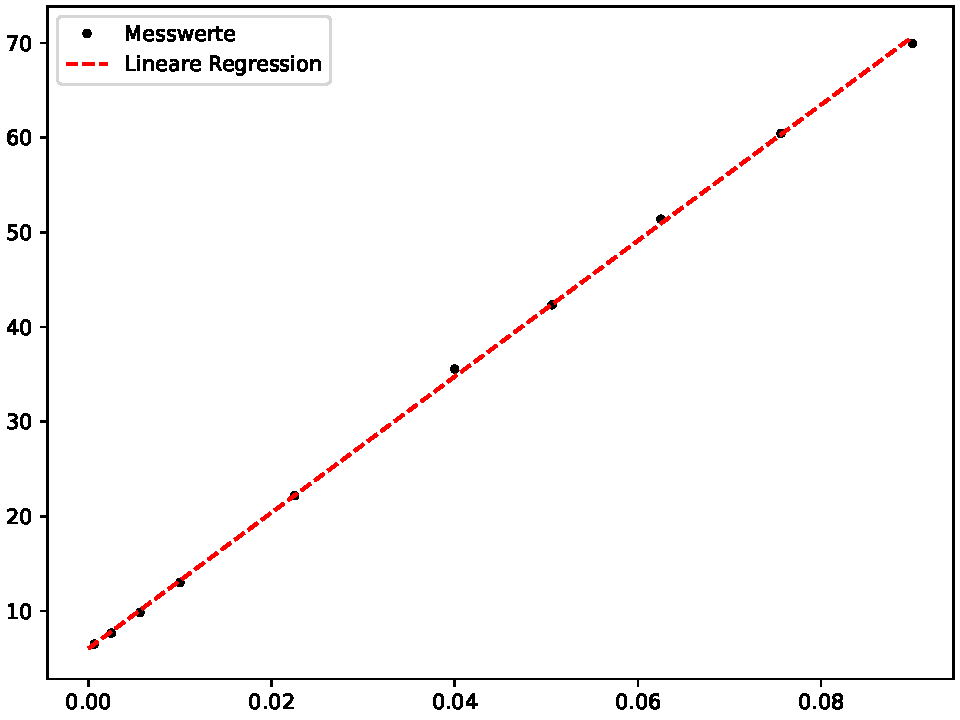
\includegraphics{plot.pdf}
    \caption{Plot.}
    \label{fig:plot}
  \end{figure}

  

  \subsection{Figuren}

  \begin{table}
    \centering
    \caption{Schwingungsdauern der Figuren mit einer Auslenkung von 90°}
    \begin{tblr}
      \colspec{S S},
      \row{1}={guard, mode=math},
      \toprule
        n & T[\unit{\seconds}] \\
      \midrule
      1 & 9.12  \\  
      2 & 9.37  \\
      3 & 9.37  \\
      4 & 9.35  \\
      5 & 9.41  \\
      \bottomrule
      Für die Kugel \\
    \end{tblr}
    \begin{tblr}
      \colspec{S S},
      \row{1}={guard, mode=math},
      \toprule
      n & T[\unit{\seconds}] \\ 
      \midrule
      1 & 9.22  \\
      2 & 9.32  \\
      3 & 9.50  \\
      4 & 9.15  \\
      5 & 9.22  \\
      \bottomrule
      Für den Zylinder \\
    \end{tblr}
  \end{table}
 
  
  Die Mittlere Periodendauer der Kugel beträgt hier$\qty{9.324(0.052)}{seconds}$
  Mithilfe von Gleichungn %\ref{eqn:Schwingungsdauer}, \ref{eqn:Eigenträgheitsmoment} 
  beträgt das Trägheitsmoment der Kugel $\qty{0.041(0.008)}{\kilo\gram\meter\squared}$ und das des
  Zylinders $\qty{0.041(0.002)}{\kilo\gram\meter\squared}$ unter beachtung des Eigenträgheitsmoments.
  
  
  
  \subsection{Trägheitsmoment der Puppe}
  Um das Trägheitsmoment der Puppe zu berechnen wurden der Kopf, der Oberkörper und die einzelnen Arme und Beine als Zylinder genähert.
  Dabie wurde die Höhe der Zylinder einmal abgemessen. 
  Der Durchmesser wurde beim Kopf über 5 und bei den anderen Körperteilen über 10, an verschiedenen Stellen gemessenen, Werte gemittelt.
